\documentclass[11pt,compress,t,notes=noshow, xcolor=table]{beamer}
\usepackage[]{graphicx}\usepackage[]{color}
% maxwidth is the original width if it is less than linewidth
% otherwise use linewidth (to make sure the graphics do not exceed the margin)
\makeatletter
\def\maxwidth{ %
  \ifdim\Gin@nat@width>\linewidth
    \linewidth
  \else
    \Gin@nat@width
  \fi
}
\makeatother

\newcommand{\citebutton}[2]{%
\beamergotobutton{\href{#2}{#1}}%
}

\newcommand{\blu}[1]{\textcolor{blue}{#1}}
\newcommand{\org}[1]{\textcolor{orange}{#1}}
\newcommand{\ques}{\textbf{\textcolor{red}{Question:  }}}
\newcommand{\questionssofar}{\begin{frame}\frametitle{Any questions?}\end{frame}}

\newcommand\warning{%
 \makebox[1.4em][c]{%
 \makebox[0pt][c]{\raisebox{.1em}{\scriptsize!}}%
 \makebox[0pt][c]{\color{red}\normalsize$\bigtriangleup$}}}%

\definecolor{fgcolor}{rgb}{0.345, 0.345, 0.345}
\newcommand{\hlnum}[1]{\textcolor[rgb]{0.686,0.059,0.569}{#1}}%
\newcommand{\hlstr}[1]{\textcolor[rgb]{0.192,0.494,0.8}{#1}}%
\newcommand{\hlcom}[1]{\textcolor[rgb]{0.678,0.584,0.686}{\textit{#1}}}%
\newcommand{\hlopt}[1]{\textcolor[rgb]{0,0,0}{#1}}%
\newcommand{\hlstd}[1]{\textcolor[rgb]{0.345,0.345,0.345}{#1}}%
\newcommand{\hlkwa}[1]{\textcolor[rgb]{0.161,0.373,0.58}{\textbf{#1}}}%
\newcommand{\hlkwb}[1]{\textcolor[rgb]{0.69,0.353,0.396}{#1}}%
\newcommand{\hlkwc}[1]{\textcolor[rgb]{0.333,0.667,0.333}{#1}}%
\newcommand{\hlkwd}[1]{\textcolor[rgb]{0.737,0.353,0.396}{\textbf{#1}}}%
\let\hlipl\hlkwb

\usepackage{framed}
\makeatletter
\newenvironment{kframe}{%
 \def\at@end@of@kframe{}%
 \ifinner\ifhmode%
  \def\at@end@of@kframe{\end{minipage}}%
  \begin{minipage}{\columnwidth}%
 \fi\fi%
 \def\FrameCommand##1{\hskip\@totalleftmargin \hskip-\fboxsep
 \colorbox{shadecolor}{##1}\hskip-\fboxsep
     % There is no \\@totalrightmargin, so:
     \hskip-\linewidth \hskip-\@totalleftmargin \hskip\columnwidth}%
 \MakeFramed {\advance\hsize-\width
   \@totalleftmargin\z@ \linewidth\hsize
   \@setminipage}}%
 {\par\unskip\endMakeFramed%
 \at@end@of@kframe}
\makeatother

\definecolor{shadecolor}{rgb}{.97, .97, .97}
\definecolor{messagecolor}{rgb}{0, 0, 0}
\definecolor{warningcolor}{rgb}{1, 0, 1}
\definecolor{errorcolor}{rgb}{1, 0, 0}
\newenvironment{knitrout}{}{} % an empty environment to be redefined in TeX

\usepackage{alltt}
\newcommand{\SweaveOpts}[1]{}  % do not interfere with LaTeX
\newcommand{\SweaveInput}[1]{} % because they are not real TeX commands
\newcommand{\Sexpr}[1]{}       % will only be parsed by R
\newcommand{\xmark}{\ding{55}}%


\usepackage[english]{babel}
\usepackage[utf8]{inputenc}

\usepackage{dsfont}
\usepackage{verbatim}
\usepackage{amsmath}
\usepackage{amsfonts}
\usepackage{amssymb}
\usepackage{bm}
\usepackage{csquotes}
\usepackage{multirow}
\usepackage{longtable}
\usepackage{booktabs}
\usepackage{enumerate}
\usepackage[absolute,overlay]{textpos}
\usepackage{psfrag}
\usepackage{algorithm}
\usepackage{algpseudocode}
\usepackage{eqnarray}
\usepackage{arydshln}
\usepackage{tabularx}
\usepackage{placeins}
\usepackage{tikz}
\usepackage{setspace}
\usepackage{colortbl}
\usepackage{mathtools}
\usepackage{wrapfig}
\usepackage{bm}
\usepackage{amsmath}
\usepackage{pifont}

\usetikzlibrary{shapes.multipart,shapes,arrows,automata,positioning,calc,chains,trees, shadows}
\tikzset{
  %Define standard arrow tip
  >=stealth',
  %Define style for boxes
  punkt/.style={
    rectangle,
    rounded corners,
    draw=black, very thick,
    text width=6.5em,
    minimum height=2em,
    text centered},
  % Define arrow style
  pil/.style={
    ->,
    thick,
    shorten <=2pt,
    shorten >=2pt,}
}

\tikzstyle{vec}=[draw, rectangle, fill = white, minimum width=5mm, minimum height=1cm, inner sep = 2pt]

\usepackage{subfig}

% Defines macros and environments
\usepackage{../../style/lmu-lecture}


\let\code=\texttt
\let\proglang=\textsf

\setkeys{Gin}{width=0.9\textwidth}

\setbeamertemplate{frametitle}{\expandafter\uppercase\expandafter\insertframetitle}

\usepackage{bbm}
% basic latex stuff
\newcommand{\pkg}[1]{{\fontseries{b}\selectfont #1}} %fontstyle for R packages
\newcommand{\lz}{\vspace{0.5cm}} %vertical space
\newcommand{\dlz}{\vspace{1cm}} %double vertical space
\newcommand{\oneliner}[1] % Oneliner for important statements
{\begin{block}{}\begin{center}\begin{Large}#1\end{Large}\end{center}\end{block}}


%new environments
\newenvironment{vbframe}  %frame with breaks and verbatim
{
 \begin{frame}[containsverbatim,allowframebreaks]
}
{
\end{frame}
}

\newenvironment{vframe}  %frame with verbatim without breaks (to avoid numbering one slided frames)
{
 \begin{frame}[containsverbatim]
}
{
\end{frame}
}

\newenvironment{blocki}[1]   % itemize block
{
 \begin{block}{#1}\begin{itemize}
}
{
\end{itemize}\end{block}
}

\newenvironment{fragileframe}[2]{  %fragile frame with framebreaks
\begin{frame}[allowframebreaks, fragile, environment = fragileframe]
\frametitle{#1}
#2}
{\end{frame}}


\newcommand{\myframe}[2]{  %short for frame with framebreaks
\begin{frame}[allowframebreaks]
\frametitle{#1}
#2
\end{frame}}

\newcommand{\remark}[1]{
  \textbf{Remark:} #1
}


\newenvironment{deleteframe}
{
\begingroup
\usebackgroundtemplate{
\includegraphics[width=\paperwidth,height=\paperheight]{../style/color/red.png}}
 \begin{frame}
}
{
\end{frame}
\endgroup
}
\newenvironment{simplifyframe}
{
\begingroup
\usebackgroundtemplate{
\includegraphics[width=\paperwidth,height=\paperheight]{../style/color/yellow.png}}
 \begin{frame}
}
{
\end{frame}
\endgroup
}\newenvironment{draftframe}
{
\begingroup
\usebackgroundtemplate{
\includegraphics[width=\paperwidth,height=\paperheight]{../style/color/green.jpg}}
 \begin{frame}
}
{
\end{frame}
\endgroup
}
% https://tex.stackexchange.com/a/261480: textcolor that works in mathmode
\makeatletter
\renewcommand*{\@textcolor}[3]{%
  \protect\leavevmode
  \begingroup
    \color#1{#2}#3%
  \endgroup
}
\makeatother





\input{../../latex-math/basic-math.tex}
\input{../../latex-math/basic-ml.tex}
\usepackage{movie15}
\usepackage{animate}

\definecolor{texblue}{rgb}{0, 0, 1}
\def\myblue#1{\textcolor{texblue}{#1}}

\newcommand{\titlefigure}{figure/sesamestreet.jpeg}
\newcommand{\learninggoals}{
\item shortcomings of BERT \& Co.
\item everything as text-to-text
\item Dynamic Masking}

\title{Using the Transformer}
% \author{}
\institute{\href{https://slds-lmu.github.io/lecture_dl4nlp/}{slds-lmu.github.io/lecture\_dl4nlp}}
\date{}

\begin{document}
\lecturechapter{T5 (Raffel et al., 2019)}
\lecture{Deep Learning for NLP}

% ------------------------------------------------------------------------------

\begin{frame}{Recap: Fine-Tuning BERT}
	\begin{figure}
	\centering
		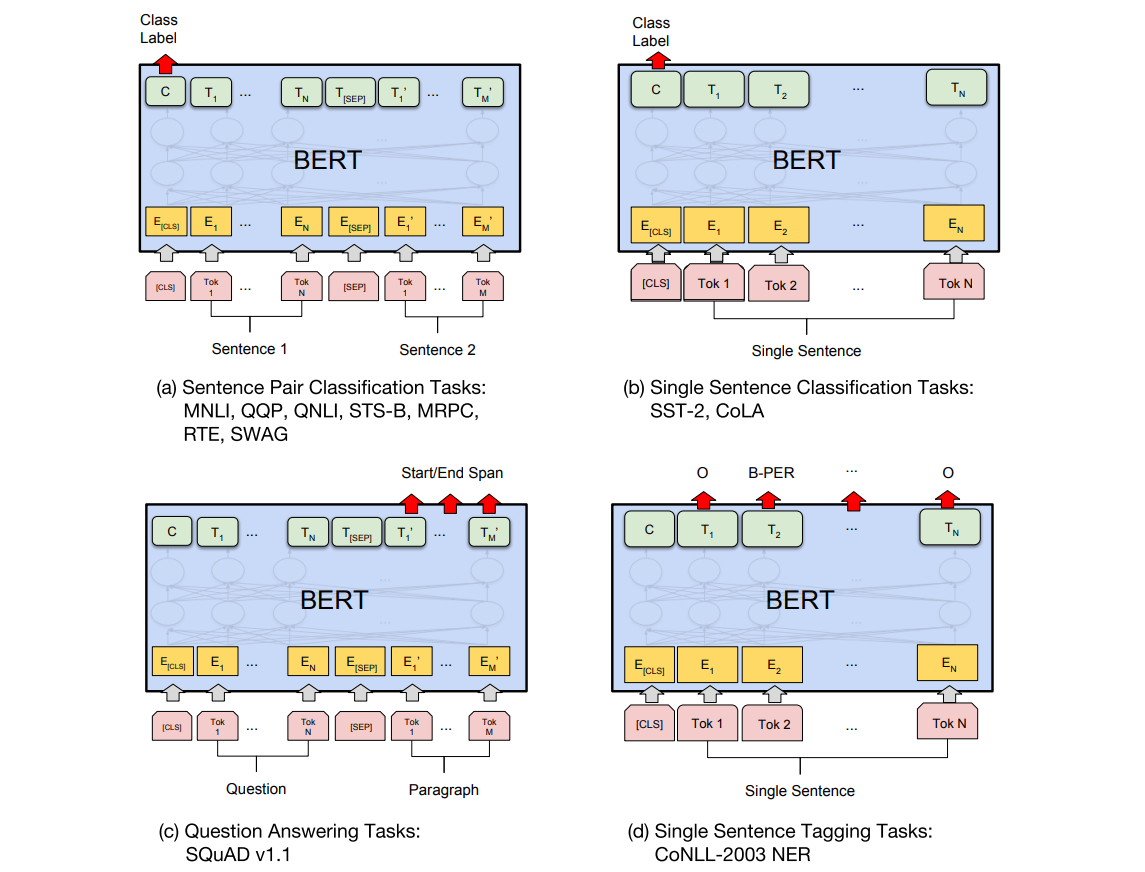
\includegraphics[width = 10cm]{../chapter04-bert/figure/bert-finetune.png}\\ 
	\citebutton{Source: Devlin et al., 2019}{https://aclanthology.org/N19-1423.pdf}
	\end{figure}
\end{frame}

% ------------------------------------------------------------------------------

\begin{frame}{Recap: BERT, RoBERTa, etc.}

\vfill

  \begin{itemize}
\item Transformer encoder
\item Training: Masked language modeling (or similar)
\item BERT* learns an enormous amount of knowledge
about language and the world through MLM training on large corpora
\item Application: fine-tune on a particular task
\item Great performance!
\item \ques What's not to like?
    \end{itemize}

\vfill

*\scriptsize{In what follows we will use BERT as a representative for this class of language models and only talk about BERT -- but the discussion includes RoBERTa, Albert, XLNet etc.}

\end{frame}

% ------------------------------------------------------------------------------

\begin{frame}{Problems with BERT (1)}

\vfill

  \begin{itemize}
\item You need a different model for each task.
\item[] (Because BERT is differently fine-tuned for each task.)
\item[] $\to$ Not realistic in many real deployment scenarios, e.g., on mobile devices.
\item \textit{Human learning:} We arguably have a \myblue{single} model that solves all tasks!
\item \ques Is there a framework that allows us to create a single model that solves all tasks?
    \end{itemize}

\vfill

\end{frame}

% ------------------------------------------------------------------------------

\begin{frame}{Problems with BERT (2)}

\vfill
			
\begin{itemize}
\item Two training modes: first (MLM) pretraining, then fine-tuning.
\item Fine-tuning is \myblue{supervised learning}, i.e., learning from labeled examples.
\item Arguably, learning from labeled examples is untypical for human learning.
\item You never learn a task solely by being presented a bunch of examples, without explanation.
\item Instead, in human learning, there is almost always a \myblue{task description}.
    \end{itemize}

\vfill

\end{frame}

% ------------------------------------------------------------------------------

\begin{frame}{Problems with BERT (2)}

\vfill
			
\begin{itemize}
\item Example: \textit{How to boil an egg.}
		\begin{itemize}
			\item ``Place eggs in the bottom of a saucepan.``
			\item ``Fill the pan with cold water.``
			\item ``Etc.``
		\end{itemize}
\item Notice that this is \myblue{not} an example but a \textit{description} of the task
\item \ques Is there a framework that allows us to leverage task descriptions?
\end{itemize}

\vfill

\end{frame}

% ------------------------------------------------------------------------------

\begin{frame}{Problems with BERT (3)}

\vfill

  \begin{itemize}
\item BERT has great performance, but \ldots
\item \ldots only if the training set is large, generally 1000s of examples
\item This is completely different from human learning!
\item We do use examples in learning, but in most cases, only a few
\end{itemize}

\vfill

\end{frame}

% ------------------------------------------------------------------------------

\begin{frame}{Problems with BERT (3)}

\vfill

  \begin{itemize}
\item Example: Maybe the person teaching you how to boil an egg will show you how to do it \textit{one or two times}
\item But probably \myblue{not} 10 times
\item Definitely \myblue{not} a 1000 times 
\item More practical concern: it's very expensive to label 1000s of examples for each task (there are many tasks).
\item \ques Is there a framework that allows us to learn from just a small number of examples?
\item This is called \myblue{few-shot learning}.
    \end{itemize}

\vfill

\end{frame}

% ------------------------------------------------------------------------------

\begin{frame}{Problems with BERT (4)}

\vfill

  \begin{itemize}
		\item More subtle aspect of the same problem (i.e., large training sets):
		\item[] $\to$ \textbf{Overfitting}
		\item Even though performance looks good on standard train/dev/test splits, the deviation between the training set and the
data actually encountered in real application can be large
		\item So our benchmarks often overestimate what performance would be in reality
  \end{itemize}

\vfill

\end{frame}

% ------------------------------------------------------------------------------

\begin{frame}{T5}

\vfill

	\textbf{Short summary:}

	\begin{itemize}
		\item \textit{Text-to-Text Transfer Transformer (T5)}
		\item A complete encoder-decoder Transformer architecture
		\item Relative positional emeddings
		\item All tasks reformulated as text-to-text tasks
		\item[$\to$] Probably the most important innovation of this work
		\item From BERT-size up to 11 Billion parameters
		\item Paradigm shift from \textit{Sequential Transfer Learning} towards \textit{Multi-Task Learning}
	\end{itemize}
	
	\vspace{.5cm}

	\begin{center}
		\href{https://1.bp.blogspot.com/-o4oiOExxq1s/Xk26XPC3haI/AAAAAAAAFU8/NBlvOWB84L0PTYy9TzZBaLf6fwPGJTR0QCLcBGAsYHQ/s1600/image3.gif}{\textbf{\beamergotobutton{Animation (Link)}}}
	\end{center}
	
\vfill

\end{frame}

% ------------------------------------------------------------------------------

\begin{frame}{Illustration}

\vfill
	
	\begin{figure}
		\centering
		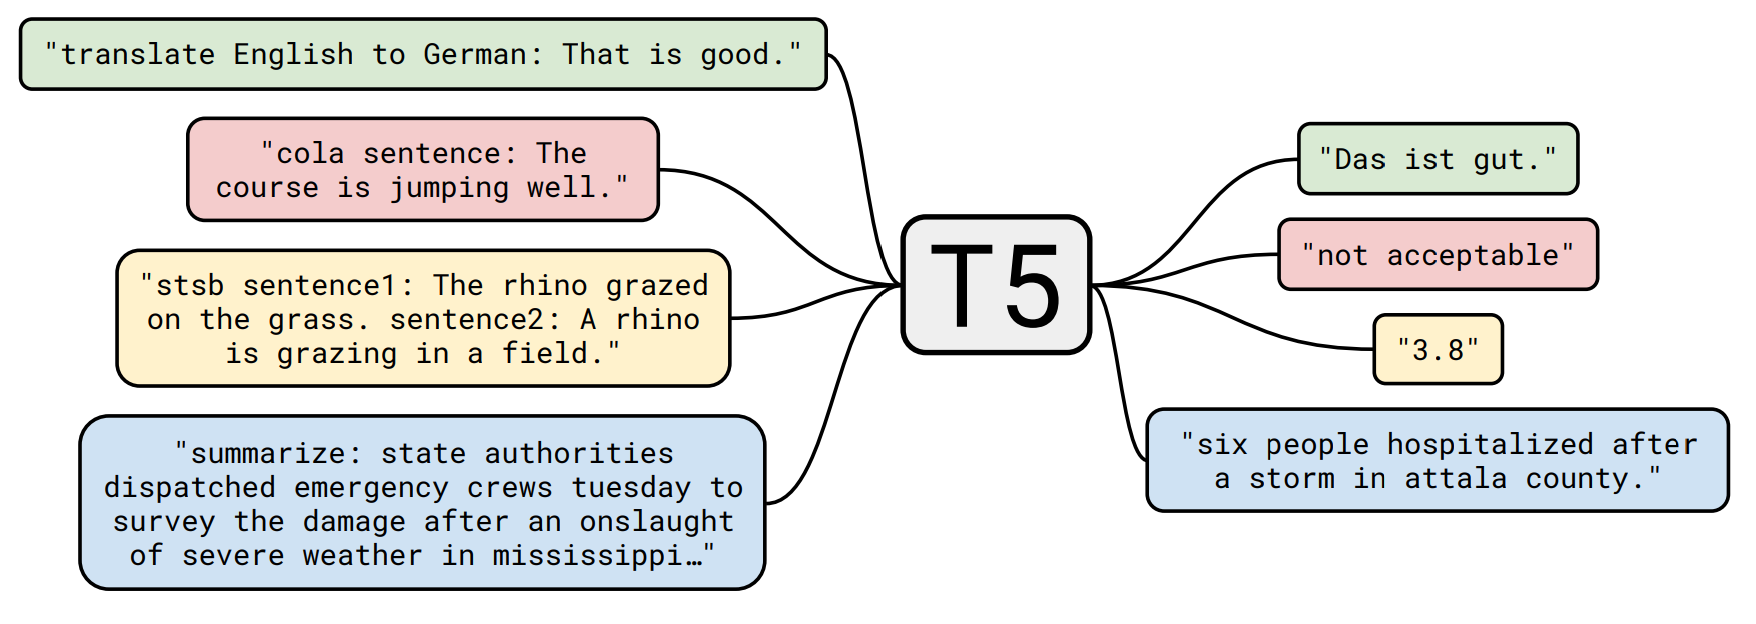
\includegraphics[width = 11cm]{figure/t5.png}\\ \citebutton{Raffel et al. (2020)}{https://jmlr.org/papers/v21/20-074.html}
	\end{figure}
	
\vfill

\end{frame}

% ------------------------------------------------------------------------------

\begin{frame}{Illustration}

\vfill
\begin{figure}
    \centering
     \animategraphics[loop,autoplay,width=10cm]{10}{figures/t5/a_}{0}{3}
\end{figure}
\vfill

\end{frame}

% ------------------------------------------------------------------------------

\begin{frame}{Input and Output Format}

\vfill

	\textbf{Input Side:}

	\begin{itemize}
		\item SentencePiece framework w/ WordPiece tokens
		\item Add task-specific (text) prefix to the original input
		\item Choice of the prefix: Hyperparameter!! 
		\item[$\to$] Changing this had limited impact
		\item[$\to$] No extensive experiments performed by the authors
	\end{itemize}
	
	\vspace{.5cm}

	\textbf{Output Side:}

	\begin{itemize}
		\item Output as a word or a piece of text (also similarity scores)
		\item If output not present in set of potential alternatives, prediction considered as wrong
	\end{itemize}
	
\vfill

\end{frame}

% ------------------------------------------------------------------------------

\begin{frame}{Add-On: Distinction to Prompting}

\vfill

	\textbf{Adding task-specific (text) prefix:}

	\begin{itemize}
		\item Add task-specific (text) prefix to the original input
		\item Model is fine-tuned on samples prepended with this prefix
		\item[$\to$] It learns to recognize what it is expected to do when encountering a specific prefix at test time
		\item[$\to$] Probably because of this: limited impact found by the authors
	\end{itemize}
	
	\vspace{.5cm}

	\textbf{Prompting:}

	\begin{itemize}
		\item Refers to just querying a trained w/o fine-tuning it (cf. next chapter)
		\item Paradigm of Few-/Zero-Shot Learning
		\item This is found to have a \textit{huge} impact on model performance
	\end{itemize}
	
\vfill

\end{frame}

% ------------------------------------------------------------------------------

\begin{frame}{Pre-training T5}

\vfill
	
	\begin{figure}
		\centering
		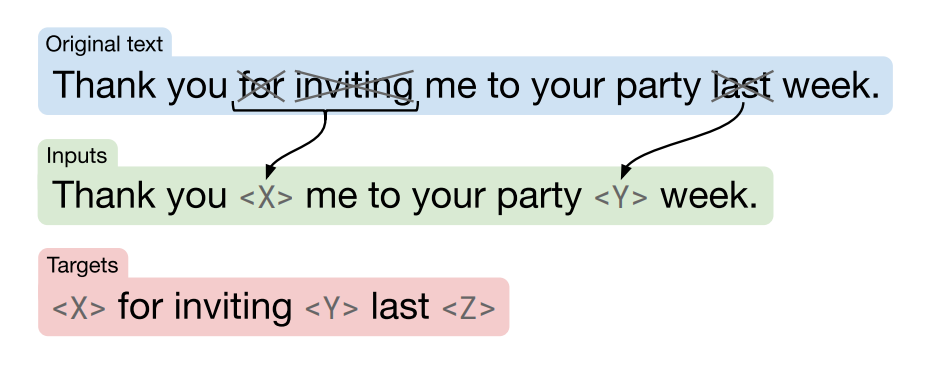
\includegraphics[width = 11cm]{figure/t5-span-pred.png}\\ 
		\footnotesize{Baseline objective (Source:} \href{https://arxiv.org/pdf/1910.10683.pdf}{\footnotesize Raffel et al., 2019)}
	\end{figure}
	
	\begin{enumerate}
		\item Mark spans in input sequence for corruptions
		\item Replace tokens with sentinel tokens
		\item Predict sentinel tokens and replaced tokens
	\end{enumerate}
	
\vfill

\end{frame}

% ------------------------------------------------------------------------------

\begin{frame}{Pre-training objectives}

\vfill

	\begin{itemize}
		\item Authors experimented with different objectives
		\item Most of them rely in some way on MLM
	\end{itemize}
	
	\begin{figure}
		\centering
		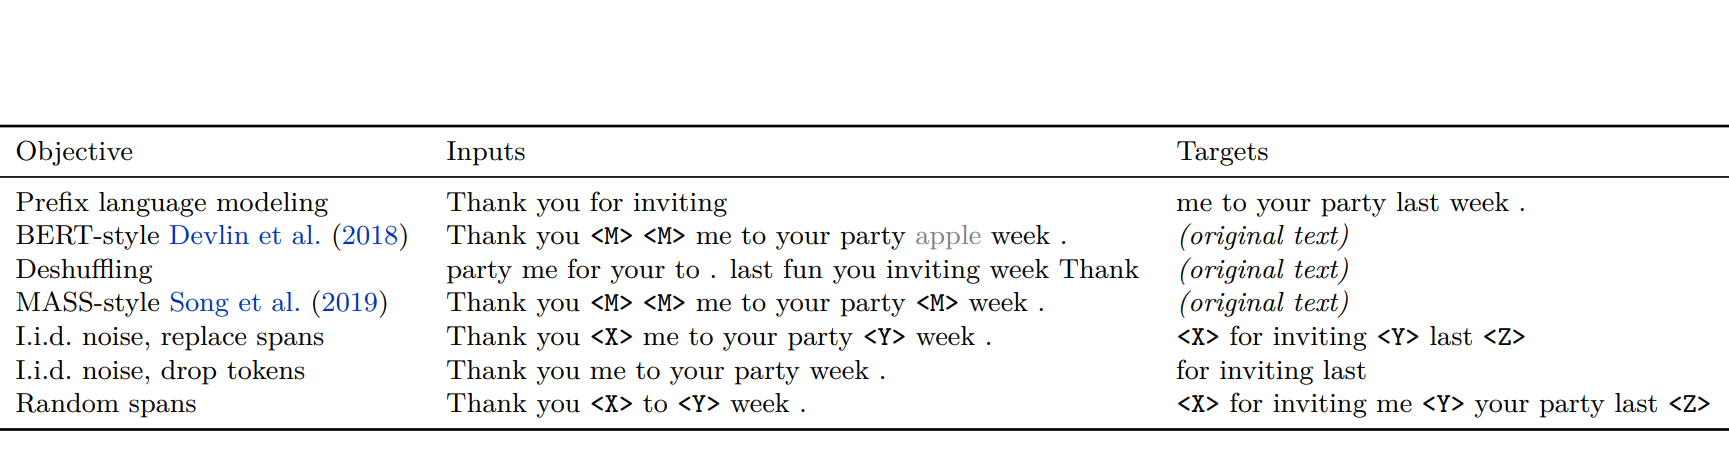
\includegraphics[width = 11cm]{figure/t5-objectives1.png}\\ 
		\footnotesize{Source:} \href{https://arxiv.org/pdf/1910.10683.pdf}{\footnotesize Raffel et al. (2019)}
	\end{figure}
	
\vfill

\end{frame}

% ------------------------------------------------------------------------------

\begin{frame}{Pre-training objectives}

\vfill

	\begin{figure}
		\centering
		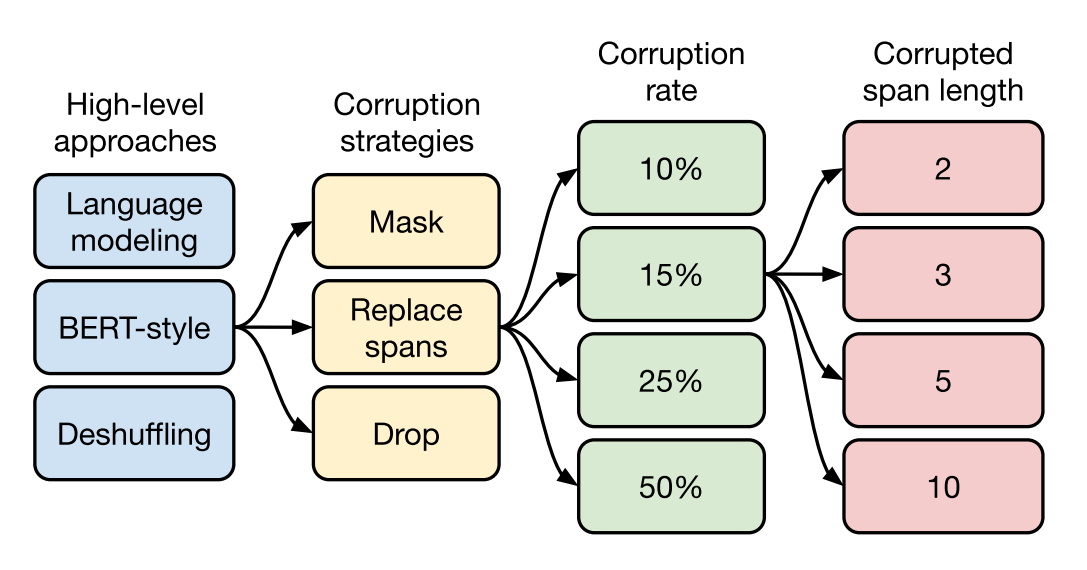
\includegraphics[width = 11cm]{figure/t5-objectives2.png}\\ 
		\footnotesize{Source:} \href{https://arxiv.org/pdf/1910.10683.pdf}{\footnotesize Raffel et al. (2019)}
	\end{figure}
	
\vfill

\end{frame}

% ------------------------------------------------------------------------------

\begin{frame}{The \textbf{C}olossal \textbf{C}lean \textbf{C}rawled \textbf{C}orpus (C4)}

\vfill

	\begin{itemize}
		\item Effort to measure the effect of quality, characteristics \& size of the pre-training resources
		\item Common Crawl as basis, careful cleaning and filtering for English language
		\item Orders of magnitude larger (750GB) compared to commonly used corpora 
	\end{itemize}
	
\vfill

\end{frame}

% ------------------------------------------------------------------------------

\begin{frame}{The \textbf{C}olossal \textbf{C}lean \textbf{C}rawled \textbf{C}orpus (C4)}

\vfill
	
	\textbf{Experiments (with respect to C4)}
	
	\begin{figure}
		\centering
		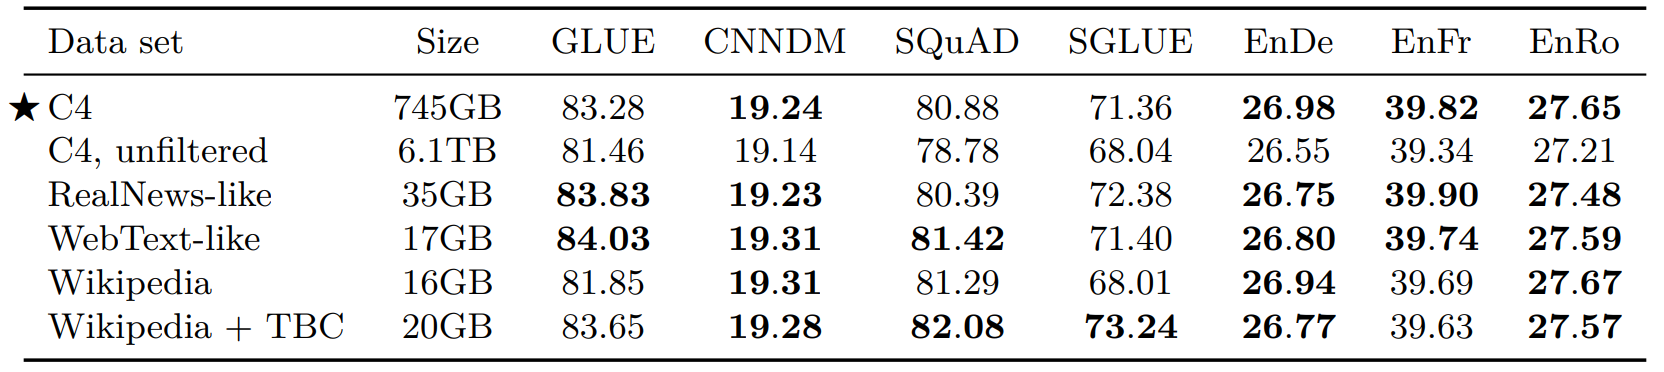
\includegraphics[width = 9cm]{figure/c4-characteristics.png}\\ 
		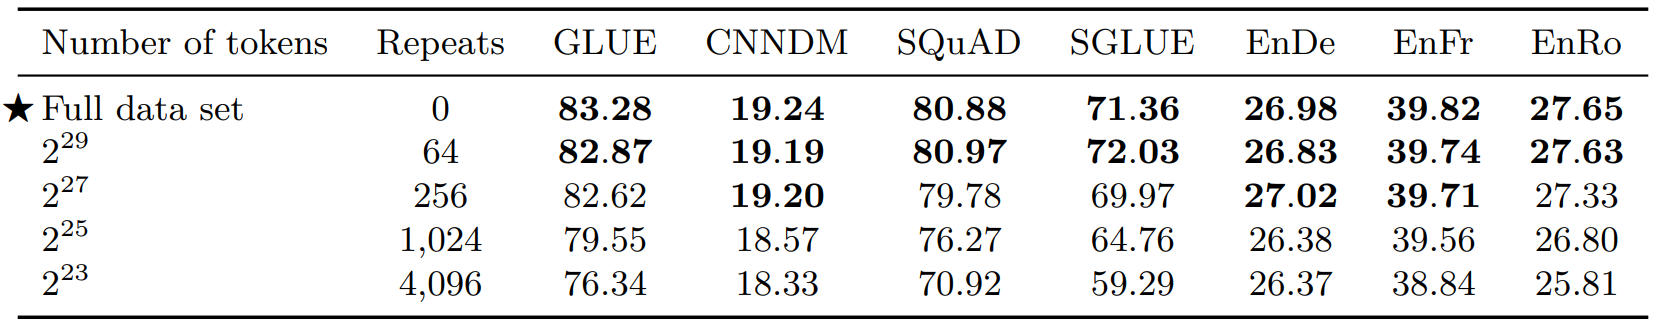
\includegraphics[width = 9cm]{figure/c4-size.png}\\ 
		\footnotesize{Source:} \href{https://arxiv.org/pdf/1910.10683.pdf}{\footnotesize Raffel et al. (2019)}
	\end{figure}
	
\vfill

\end{frame}

% ------------------------------------------------------------------------------

\begin{frame}{T5 - Exhaustive Experiments}

\vfill

	\textbf{Performed experiments with respect to ..}
	
	\begin{itemize}
		\item \textit{.. architecture, size \& objective}
		\item[$\to$] enc, dec, enc-dec
		\item[$\to$] Between 60M and 11B parameters
		\item \textit{.. details of the Denoising objective (which was found to work best)}
		\item \textit{.. fine-tuning methods}
		\item[$\to$] Adapter layers
		\item[$\to$] Gradual Unfreezing (cf. ULMFiT)
		\item \textit{.. Multi-task learning strategies}
		\item[$\to$] Examples-proportional mixing
		\item[$\to$] Temperature-scaled mixing
	\end{itemize}
	
\vfill

\end{frame}

% ------------------------------------------------------------------------------

\begin{frame}{Benchmark results}

\vfill

	\begin{figure}
		\centering
		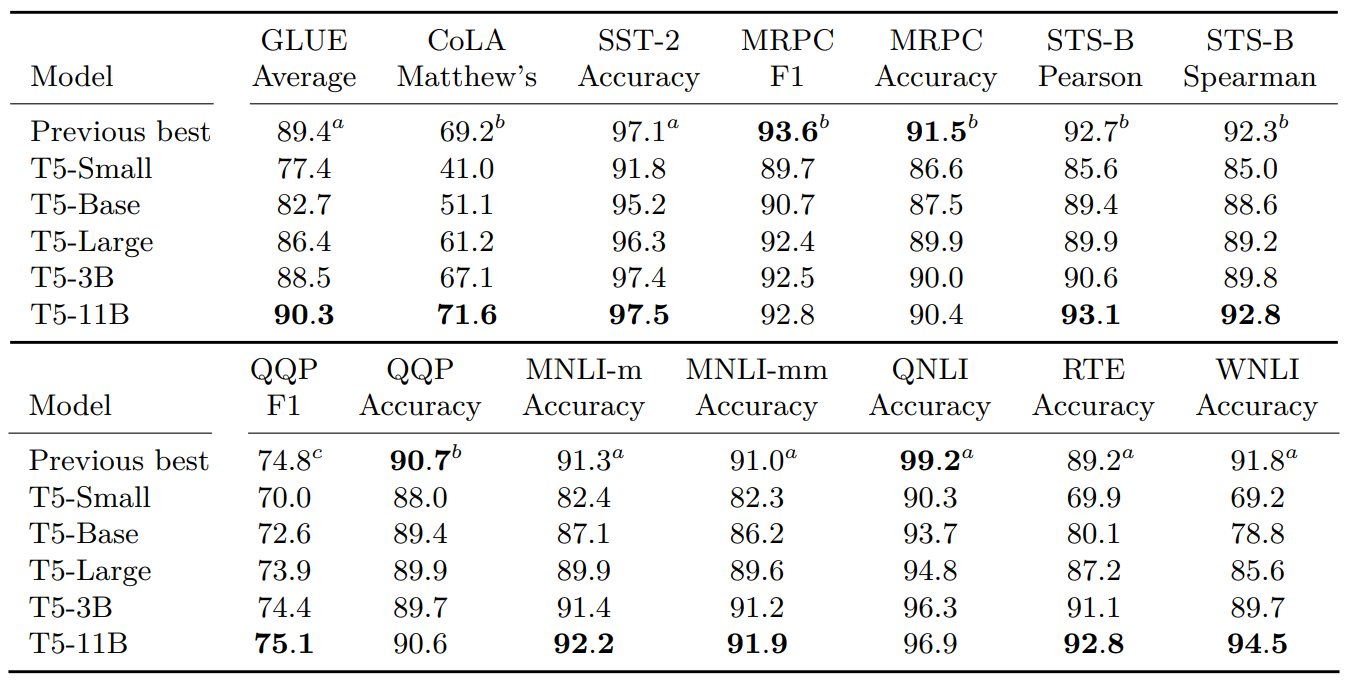
\includegraphics[width = 9cm]{figure/t5-glue.png}\\ 
		\footnotesize{Results on GLUE (Source:} \href{https://arxiv.org/pdf/1910.10683.pdf}{\footnotesize Raffel et al., 2019)}
	\end{figure}
	
\vfill

\end{frame}

% ------------------------------------------------------------------------------

\begin{frame}{Benchmark results}

\vfill

	\begin{figure}
		\centering
		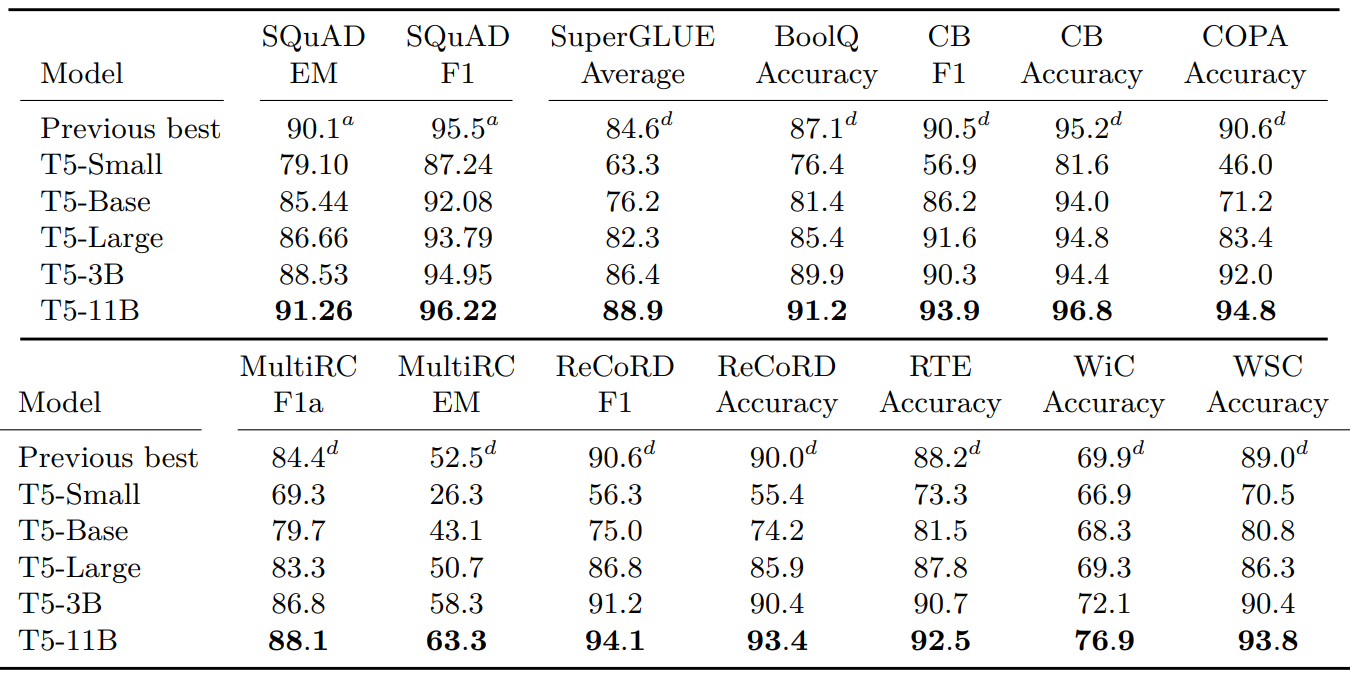
\includegraphics[width = 9cm]{figure/t5-squad-sglue.png}\\ 
		\footnotesize{Results on SQUAD and S-GLUE (Source:} \href{https://arxiv.org/pdf/1910.10683.pdf}{\footnotesize Raffel et al., 2019)}
	\end{figure}
	
\vfill

\end{frame}

% ------------------------------------------------------------------------------

\begin{frame}{Benchmark results}

\vfill

	\begin{figure}
		\centering
		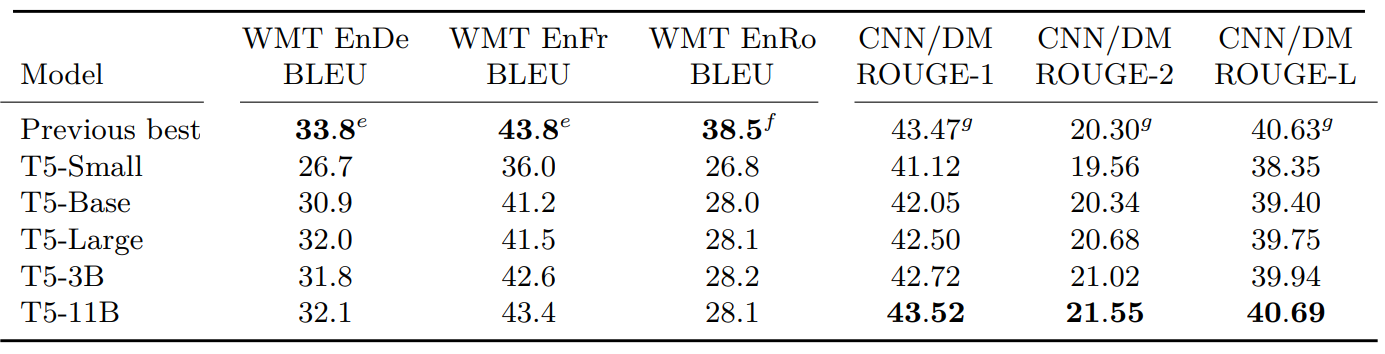
\includegraphics[width = 9cm]{figure/t5-mt.png}\\ 
		\footnotesize{Results on MT/Summarization Benchmarks (Source:} \href{https://arxiv.org/pdf/1910.10683.pdf}{\footnotesize Raffel et al., 2019)}
	\end{figure}
	
\vfill

\end{frame}

% ------------------------------------------------------------------------------

\begin{frame}{T5 - Exhaustive Experiments}

\vfill
	
	\textbf{Conclusions}
	
	\begin{itemize}
		\item Encoder-decoder architecture works best in this "text-to-text" setting
		\item More data, larger models \& ensembling all boost the performance
			\begin{itemize}
				\item Larger models trained for fewer steps better than smaller models on more data
				\item Ensembling: Using same base pre-trained models worse than complete separate model ensembles
			\end{itemize}
		\item Different denoising objectives work similarly well
		\item Updating \textit{all} model parameters during fine-tuning works best (but expensive)
	\end{itemize}
	
\vfill

\end{frame}

% ------------------------------------------------------------------------------

\endlecture
\end{document}
